% Options for packages loaded elsewhere
\PassOptionsToPackage{unicode}{hyperref}
\PassOptionsToPackage{hyphens}{url}
%
\documentclass[
]{article}
\usepackage{lmodern}
\usepackage{amssymb,amsmath}
\usepackage{ifxetex,ifluatex}
\ifnum 0\ifxetex 1\fi\ifluatex 1\fi=0 % if pdftex
  \usepackage[T1]{fontenc}
  \usepackage[utf8]{inputenc}
  \usepackage{textcomp} % provide euro and other symbols
\else % if luatex or xetex
  \usepackage{unicode-math}
  \defaultfontfeatures{Scale=MatchLowercase}
  \defaultfontfeatures[\rmfamily]{Ligatures=TeX,Scale=1}
\fi
% Use upquote if available, for straight quotes in verbatim environments
\IfFileExists{upquote.sty}{\usepackage{upquote}}{}
\IfFileExists{microtype.sty}{% use microtype if available
  \usepackage[]{microtype}
  \UseMicrotypeSet[protrusion]{basicmath} % disable protrusion for tt fonts
}{}
\makeatletter
\@ifundefined{KOMAClassName}{% if non-KOMA class
  \IfFileExists{parskip.sty}{%
    \usepackage{parskip}
  }{% else
    \setlength{\parindent}{0pt}
    \setlength{\parskip}{6pt plus 2pt minus 1pt}}
}{% if KOMA class
  \KOMAoptions{parskip=half}}
\makeatother
\usepackage{xcolor}
\IfFileExists{xurl.sty}{\usepackage{xurl}}{} % add URL line breaks if available
\IfFileExists{bookmark.sty}{\usepackage{bookmark}}{\usepackage{hyperref}}
\hypersetup{
  pdftitle={webdata\_rus.md},
  hidelinks,
  pdfcreator={LaTeX via pandoc}}
\urlstyle{same} % disable monospaced font for URLs
\usepackage{color}
\usepackage{fancyvrb}
\newcommand{\VerbBar}{|}
\newcommand{\VERB}{\Verb[commandchars=\\\{\}]}
\DefineVerbatimEnvironment{Highlighting}{Verbatim}{commandchars=\\\{\}}
% Add ',fontsize=\small' for more characters per line
\newenvironment{Shaded}{}{}
\newcommand{\AlertTok}[1]{\textcolor[rgb]{1.00,0.00,0.00}{\textbf{#1}}}
\newcommand{\AnnotationTok}[1]{\textcolor[rgb]{0.38,0.63,0.69}{\textbf{\textit{#1}}}}
\newcommand{\AttributeTok}[1]{\textcolor[rgb]{0.49,0.56,0.16}{#1}}
\newcommand{\BaseNTok}[1]{\textcolor[rgb]{0.25,0.63,0.44}{#1}}
\newcommand{\BuiltInTok}[1]{#1}
\newcommand{\CharTok}[1]{\textcolor[rgb]{0.25,0.44,0.63}{#1}}
\newcommand{\CommentTok}[1]{\textcolor[rgb]{0.38,0.63,0.69}{\textit{#1}}}
\newcommand{\CommentVarTok}[1]{\textcolor[rgb]{0.38,0.63,0.69}{\textbf{\textit{#1}}}}
\newcommand{\ConstantTok}[1]{\textcolor[rgb]{0.53,0.00,0.00}{#1}}
\newcommand{\ControlFlowTok}[1]{\textcolor[rgb]{0.00,0.44,0.13}{\textbf{#1}}}
\newcommand{\DataTypeTok}[1]{\textcolor[rgb]{0.56,0.13,0.00}{#1}}
\newcommand{\DecValTok}[1]{\textcolor[rgb]{0.25,0.63,0.44}{#1}}
\newcommand{\DocumentationTok}[1]{\textcolor[rgb]{0.73,0.13,0.13}{\textit{#1}}}
\newcommand{\ErrorTok}[1]{\textcolor[rgb]{1.00,0.00,0.00}{\textbf{#1}}}
\newcommand{\ExtensionTok}[1]{#1}
\newcommand{\FloatTok}[1]{\textcolor[rgb]{0.25,0.63,0.44}{#1}}
\newcommand{\FunctionTok}[1]{\textcolor[rgb]{0.02,0.16,0.49}{#1}}
\newcommand{\ImportTok}[1]{#1}
\newcommand{\InformationTok}[1]{\textcolor[rgb]{0.38,0.63,0.69}{\textbf{\textit{#1}}}}
\newcommand{\KeywordTok}[1]{\textcolor[rgb]{0.00,0.44,0.13}{\textbf{#1}}}
\newcommand{\NormalTok}[1]{#1}
\newcommand{\OperatorTok}[1]{\textcolor[rgb]{0.40,0.40,0.40}{#1}}
\newcommand{\OtherTok}[1]{\textcolor[rgb]{0.00,0.44,0.13}{#1}}
\newcommand{\PreprocessorTok}[1]{\textcolor[rgb]{0.74,0.48,0.00}{#1}}
\newcommand{\RegionMarkerTok}[1]{#1}
\newcommand{\SpecialCharTok}[1]{\textcolor[rgb]{0.25,0.44,0.63}{#1}}
\newcommand{\SpecialStringTok}[1]{\textcolor[rgb]{0.73,0.40,0.53}{#1}}
\newcommand{\StringTok}[1]{\textcolor[rgb]{0.25,0.44,0.63}{#1}}
\newcommand{\VariableTok}[1]{\textcolor[rgb]{0.10,0.09,0.49}{#1}}
\newcommand{\VerbatimStringTok}[1]{\textcolor[rgb]{0.25,0.44,0.63}{#1}}
\newcommand{\WarningTok}[1]{\textcolor[rgb]{0.38,0.63,0.69}{\textbf{\textit{#1}}}}
\usepackage{longtable,booktabs}
% Correct order of tables after \paragraph or \subparagraph
\usepackage{etoolbox}
\makeatletter
\patchcmd\longtable{\par}{\if@noskipsec\mbox{}\fi\par}{}{}
\makeatother
% Allow footnotes in longtable head/foot
\IfFileExists{footnotehyper.sty}{\usepackage{footnotehyper}}{\usepackage{footnote}}
\makesavenoteenv{longtable}
\usepackage{graphicx}
\makeatletter
\def\maxwidth{\ifdim\Gin@nat@width>\linewidth\linewidth\else\Gin@nat@width\fi}
\def\maxheight{\ifdim\Gin@nat@height>\textheight\textheight\else\Gin@nat@height\fi}
\makeatother
% Scale images if necessary, so that they will not overflow the page
% margins by default, and it is still possible to overwrite the defaults
% using explicit options in \includegraphics[width, height, ...]{}
\setkeys{Gin}{width=\maxwidth,height=\maxheight,keepaspectratio}
% Set default figure placement to htbp
\makeatletter
\def\fps@figure{htbp}
\makeatother
\setlength{\emergencystretch}{3em} % prevent overfull lines
\providecommand{\tightlist}{%
  \setlength{\itemsep}{0pt}\setlength{\parskip}{0pt}}
\setcounter{secnumdepth}{-\maxdimen} % remove section numbering

\title{webdata\_rus.md}
\author{}
\date{}

\begin{document}
\maketitle

\hypertarget{header-n2623}{%
\section[Форматы веб-данных в Lazarus/FPC.]{\texorpdfstring{Форматы
веб-данных в
Lazarus/FPC.\footnote{Данная статья является переводом статьи Michaël
  Van Canneyt ``Web data formats in Lazarus/FPC'', оригинальный текст
  которой можно увидеть здесь
  https://www.freepascal.org/\textasciitilde michael/articles/webdata/webdata.pdf.
  Автор любезно предоставил свое разрешение на свободное распространение
  данного перевода при условии предоставлении ему полного текста.}}{Форматы веб-данных в Lazarus/FPC.}}\label{header-n2623}}

Michaël Van Canneyt, 30 июня 2018г.

(перевод Zoltanleo, aka Док)

\textbf{Аннотация}. В наши дни трудно избежать контакта с популярными
форматами веб-данных, такими как XML и - совсем недавно - JSON. К
счастью, Lazarus и FPC оснащены набором инструментов для обработки и
вывода этих форматов. Обзор.

\hypertarget{header-n2416}{%
\subsection{Вступление.}\label{header-n2416}}

В эпоху, когда такие слова, как SOA, Webservices и SOAP и AJAX считаются
стандартными инструментами каждого программиста, трудно избежать
строительных блоков, на которых построены эти концепции. Формат данных
XML является краеугольным камнем, на котором строятся эти технологии:
текстовый формат кодирования и структурирования данных. Он сильно
стандартизирован консорциумом W3, который сделал его форматом выбора для
передачи данных. FPC/Lazarus поставляется с набором инструментов,
которые реализуют некоторые стандарты и рекомендации консорциума W3:
DOM, XPath.

По мере того, как стандарты \texttt{XML} становятся все более и более
сложными - и, следовательно, громоздкими - \texttt{JSON} (JavaScript
Object Notation) стал вторым стандартом для формата данных: он подходит
в первую очередь для передачи данных в веб-браузер, где JavaScript можно
легко разобрать и использовать как родной способ чтения данных: сам
движок JavaScript может быть использован для анализа данных и
преобразования их в javascript.

В то время как обозначение \texttt{JSON} для данных на самом деле
бесполезно за пределами браузера, веб-сервер приложение должно быть в
состоянии генерировать его, так чтобы браузер мог прочитать его. Помимо
(чрезвычайно простых) спецификаций формата, существует немного
стандартов, которые должны быть реализованы, поэтому реализация JSON FPC
была создана таким образом, чтобы данные, которые необходимо отправить,
были просты в создании и обработке.

В этой статье будут обсуждаться реализации, доступные в FPC/Lazarus для
обработки \texttt{XML} и \texttt{JSON}. Обсуждаться будут не сами
форматы XML и JSON, а только как именно эти форматы можно обрабатывать.

\hypertarget{header-n2422}{%
\subsection{XML: способ DOM.}\label{header-n2422}}

Консорциум W3 создал спецификацию для представления XML-документа в
памяти: \texttt{DOM} (\textsuperscript{англ.}Document Object Model, или
\textsuperscript{рус.}объектная модель документа)\footnote{https://www.w3.org/TR/REC-DOM-Level-1}
. Free Pascal содержит реализацию DOM Level 1 (с некоторыми расширениями
DOM level 2) в модуле \texttt{DOM}. Работать с \texttt{DOM} легко, но
требуется, чтобы документ всегда был полностью в памяти.

DOM представляет документ \texttt{XML} в виде дерева узлов (класса
\texttt{TDomNode}): все части документа описываются с использованием
потомков TDOMNode. Какую это часть, видно из свойства \texttt{NodeType}
класса \texttt{TDOMNode}: у каждого потомка есть свое значение
\texttt{NodeType}. Основные потомки \texttt{TDOMNode} с их
\texttt{NodeTypes} можно найти в таблице 1.

\textbf{Таблица 1: Основные типы и их типы узлов}

\begin{longtable}[]{@{}lll@{}}
\toprule
\textbf{Класс} & \textbf{Тип узла} & \textbf{Представляемые ими
данные}\tabularnewline
\midrule
\endhead
\textbf{TDOMElement} & ELEMENT\_NODE & тэг XML\tabularnewline
\textbf{TDOMAttr} & ATTRIBUTE\_NODE & атрибут тэга XML\tabularnewline
\textbf{TDOMText} & TEXT\_NODE & текст, заключенный в тэги
XML\tabularnewline
\textbf{TDOMComment} & TEXT\_NODE & XML-комментарий\tabularnewline
\textbf{TDOMCDATASection} & CDATA\emph{SECTION}NODE & раздел
CDATA\tabularnewline
\bottomrule
\end{longtable}

Каждый узел может иметь несколько дочерних узлов, и дерево узлов можно
полностью просмотреть с помощью следующих методов функции
\texttt{TDOMNode}:

\begin{itemize}
\item
  \texttt{FirstChild} возвращает первый дочерний элемент
  \texttt{TDOMNode}.
\item
  \texttt{LastChild} возвращает последнего потомка \texttt{TDOMNode}.
\item
  \texttt{NextSibling} возвращает следующий узел на том же уровне
  текущего \texttt{TDOMNode}.
\item
  \texttt{PreviousSibling} возвращает предыдущий узел на том же уровне
  текущего \texttt{TDOMNode}.
\end{itemize}

Полный документ \texttt{XML} представлен классом \texttt{TDOMLDocument}.
Он содержит свойство \texttt{DocumentElement}, которое имеет тип
\texttt{TDOMElement}, и содержит экземпляр первого элемента в документе
XML. Класс \texttt{TDOMNode} содержит свойство \texttt{OwnerDocument},
которое указывает на экземпляр \texttt{TDOMDocument}, частью которого он
является. Потомок \texttt{TXMLDocumen}t имеет некоторые дополнительные
свойства для описания кодировки, таблицы стилей и т. Д. В дальнейшем
будет использоваться \texttt{TXMLDocument}, но большинство методов
фактически определены в \texttt{TDOMDocument}.

Поскольку экземпляр \texttt{TXMLDocument} является владельцем всех
узлов, он также отвечает за создание узлов. Для этого есть следующие
методы создания узлов:

\begin{Shaded}
\begin{Highlighting}[]
\KeywordTok{function}\NormalTok{ CreateElement(}\KeywordTok{const}\NormalTok{ tagName: DOMString): TDOMElement; }
\KeywordTok{function}\NormalTok{ CreateTextNode(}\KeywordTok{const}\NormalTok{ data: DOMString): TDOMText; }
\KeywordTok{function}\NormalTok{ CreateComment(}\KeywordTok{const}\NormalTok{ data: DOMString): TDOMComment; }
\KeywordTok{function}\NormalTok{ CreateCDATASection(}\KeywordTok{const}\NormalTok{ data: DOMString): TDOMCDATASection; }
\KeywordTok{function}\NormalTok{ CreateAttribute(}\KeywordTok{const}\NormalTok{ name: DOMString): TDOMAttr;}
\end{Highlighting}
\end{Shaded}

После создания узла его можно вставить в дерево документа одним из
следующих методов \texttt{TDOMNode}:

\begin{Shaded}
\begin{Highlighting}[]
\KeywordTok{function}\NormalTok{ InsertBefore(NewChild, RefChild: TDOMNode): TDOMNode; }
\KeywordTok{function}\NormalTok{ ReplaceChild(NewChild, OldChild: TDOMNode): TDOMNode; }
\KeywordTok{function}\NormalTok{ RemoveChild(OldChild: TDOMNode): TDOMNode; }
\KeywordTok{function}\NormalTok{ AppendChild(NewChild: TDOMNode): TDOMNode;}
\end{Highlighting}
\end{Shaded}

Вооружившись приведенными выше определениями, можно сделать простое
приложение для просмотра и редактирования документа \texttt{XML}.
Логично представить XML-документ в виде древовидной структуры с
элементами и текстами в качестве узлов в дереве.

\hypertarget{header-n2468}{%
\subsection{Простой просмотрщик XML.}\label{header-n2468}}

Приложение для просмотра \texttt{XML} состоит из единой формы с меню,
которое содержит обычные пункты меню файлов (новый, открыть, сохранить и
«сохранить как»), и панели инструментов с теми же двумя действиями, что
и у меню. Оставшаяся часть формы заполнена экземпляром
\texttt{TTreeView} (TVXML), который покажет документ \texttt{XML}, и
экземпляром \texttt{TPanel} (PDetails), который будет использоваться для
отображения сведений о текущем узле.

Чтобы заполнить древовидную структуру содержимым \texttt{TXMLDocument},
воспользуемся следующим кодом:

\begin{Shaded}
\begin{Highlighting}[]
\KeywordTok{procedure}\NormalTok{ TMainForm.ShowDocument(AXML: TXMLDocument); }
\KeywordTok{begin} 
  \KeywordTok{with}\NormalTok{ TVXML.Items }\KeywordTok{do} 
  \KeywordTok{begin} 
\NormalTok{    BeginUpdate; }
    \KeywordTok{try} 
\NormalTok{      Clear; }
      \KeywordTok{if}\NormalTok{ Assigned(AXML.DocumentElement) }\KeywordTok{then} 
      \KeywordTok{begin} 
\NormalTok{        ShowNode(}\KeywordTok{Nil}\NormalTok{,AXML.DocumentElement);}
\NormalTok{        TVXML.Selected:=TVXML.Items.GetFirstNode; }
      \KeywordTok{end}\NormalTok{; }
    \KeywordTok{finally} 
\NormalTok{      EndUpdate; }
    \KeywordTok{end}\NormalTok{;}
  \KeywordTok{end}\NormalTok{; }
\KeywordTok{end}\NormalTok{;}
\end{Highlighting}
\end{Shaded}

Код довольно прост: он очищает древовидную структуру, а затем позволяет
методу \texttt{ShowNode} выполнять фактическую работу, начиная с узла
\texttt{DocumentElement}. \texttt{ShowNode} - это простая процедура с
рекурсией:

\begin{Shaded}
\begin{Highlighting}[]
\KeywordTok{procedure}\NormalTok{ TMainForm.ShowNode(AParent: TTreeNode; E: TDomNode);}
\KeywordTok{var}
\NormalTok{  N: TTreeNode;}
\NormalTok{  D: TDomNode;}
\KeywordTok{begin}
\NormalTok{  N:= TVXML.Items.AddChild(AParent,E.NodeName);}
\NormalTok{  N.Data:= E;}
\NormalTok{  D:= E.FirstChild;}

  \KeywordTok{while}\NormalTok{ (D \textless{}\textgreater{} }\KeywordTok{nil}\NormalTok{) }\KeywordTok{do}
  \KeywordTok{begin}
    \KeywordTok{case}\NormalTok{ D.NodeType }\KeywordTok{of}
\NormalTok{      ELEMENT\_NODE: ShowNode(N,D);}
\NormalTok{         TEXT\_NODE: ShowNode(N,D);}
    \KeywordTok{end}\NormalTok{;}
\NormalTok{    D:= D.NextSibling;}
  \KeywordTok{end}\NormalTok{;}
\KeywordTok{end}\NormalTok{;}
\end{Highlighting}
\end{Shaded}

Первое, что делается, это создается узел в древовидном представлении для
отображения \texttt{TDOMNode}. Свойство \texttt{NodeName} используется в
качестве текста для узла. Для экземпляра \texttt{TDOMElement} это имя
тега. Для экземпляра \texttt{TDOMText} это фиксированный текст
\texttt{\#text}. После этого дочерние узлы просматриваются с помощью
\texttt{FirstChild} и \texttt{NextSibling}, и они добавляются во вновь
созданный узел, вызывая \texttt{ShowNode}. Обратите внимание, что
\texttt{ShowNode} вызывается только для дочерних узлов типа
\texttt{ELEMENT\_NODE} и \texttt{TEXT\_NODE}. Это означает, что атрибуты
не отображаются в дереве.

Вышеупомянутых двух коротких процедур достаточно, чтобы отобразить
XML-документ в TreeView. Для отображения содержимого узла используется
панель. Когда узел выбран в дереве, происходит
событие\texttt{OnSelectionChanged}:

\begin{Shaded}
\begin{Highlighting}[]
\KeywordTok{procedure}\NormalTok{ TMainForm.TVXMLSelectionChanged(Sender: TObject);}
\KeywordTok{begin}
\NormalTok{  ClearNodeData;}
  \KeywordTok{if}\NormalTok{ Assigned(TVXML.Selected) }\KeywordTok{and}\NormalTok{ Assigned(TVXML.Selected.Data) }\KeywordTok{then}
\NormalTok{    ShowNodeData(TDomNode(TVXML.Selected.Data))}
    \KeywordTok{else}
\NormalTok{    PDetails.Caption:=SSelectNode;}
\KeywordTok{end}\NormalTok{;}
\end{Highlighting}
\end{Shaded}

\texttt{ClearNodeData} очищает содержимое панели \texttt{PDetails},
удаляя все элементы управления в ней:

\begin{Shaded}
\begin{Highlighting}[]
\KeywordTok{procedure}\NormalTok{ TMainForm.ClearNodeData;}
\KeywordTok{begin}
  \KeywordTok{with}\NormalTok{ PDetails }\KeywordTok{do}
    \KeywordTok{while}\NormalTok{ (ControlCount \textgreater{} }\DecValTok{0}\NormalTok{) }\KeywordTok{do}\NormalTok{ Controls[}\DecValTok{0}\NormalTok{].Free;}
\KeywordTok{end}\NormalTok{;}
\end{Highlighting}
\end{Shaded}

Элементы управления на панели \texttt{PDetails} создаются кодом в вызове
\texttt{ShowNodeData}, где также создается путь к текущему узлу и
отображается в строке состояния:

\begin{Shaded}
\begin{Highlighting}[]
\KeywordTok{procedure}\NormalTok{ TMainForm.ShowNodeData(N: TDomNode);}
\KeywordTok{var}
\NormalTok{  P: TDomNode;}
\NormalTok{  S: }\DataTypeTok{String}\NormalTok{;}
\KeywordTok{begin}
\NormalTok{  PDetails.Caption:= }\StringTok{\textquotesingle{}\textquotesingle{}}\NormalTok{;}
\NormalTok{  P:= N;}
\NormalTok{  S:= }\StringTok{\textquotesingle{}\textquotesingle{}}\NormalTok{;}
  \KeywordTok{while}\NormalTok{ (P \textless{}\textgreater{} }\KeywordTok{nil}\NormalTok{) }\KeywordTok{and} \KeywordTok{not}\NormalTok{ (P }\KeywordTok{is}\NormalTok{ TXMLDocument) }\KeywordTok{do}
  \KeywordTok{begin}
    \KeywordTok{if}\NormalTok{ S \textless{}\textgreater{} }\StringTok{\textquotesingle{}\textquotesingle{}} \KeywordTok{then}\NormalTok{ S:= }\StringTok{\textquotesingle{}/\textquotesingle{}}\NormalTok{ + S;}
\NormalTok{    S:= P.NodeName + S;}
\NormalTok{    P:= P.ParentNode;}
  \KeywordTok{end}\NormalTok{;}

\NormalTok{  SBXML.SimpleText:= Format(SCurrentNode,[S]);}

  \KeywordTok{case}\NormalTok{ N.NodeType }\KeywordTok{of}
\NormalTok{       TEXT\_NODE: ShowTextData(N }\KeywordTok{as}\NormalTok{ TDomText);}
\NormalTok{    ELEMENT\_NODE: ShowElementData(N }\KeywordTok{as}\NormalTok{ TDomElement);}
  \KeywordTok{end}\NormalTok{;}
\KeywordTok{end}\NormalTok{;}
\end{Highlighting}
\end{Shaded}

Как видно, для текстового узла реальная работа происходит в вызове
\texttt{ShowTextData}:

\begin{Shaded}
\begin{Highlighting}[]
\KeywordTok{procedure}\NormalTok{ TMainForm.ShowTextData(N: TDomNode);}
\KeywordTok{var}
\NormalTok{  M: TMemo;}
\KeywordTok{begin}
\NormalTok{  DataTopLabel(SNodeText);}
\NormalTok{  M:= TMemo.Create(}\KeywordTok{Self}\NormalTok{);}
\NormalTok{  M.Parent:= PDetails;}
\NormalTok{  M.Lines.}\DataTypeTok{Text}\NormalTok{:= N.NodeValue;}
\NormalTok{  M.Align:= alClient;}
\KeywordTok{end}\NormalTok{;}
\end{Highlighting}
\end{Shaded}

Процедура \texttt{DataTopLabel} показывает метку, выровненную по
верхнему краю панели \texttt{PDetail}. Остальная часть кода показывает
\texttt{TMemo} в остальной части панели и устанавливает его текст в
свойстве \texttt{NodeValue} \texttt{TDOMNode}. Для текстового узла это
фактический текст узла.

Вызов \texttt{ShowElementData}, используемый для отображения элемента
\texttt{TDOME}, немного сложнее, поскольку он должен отображать все
атрибуты элемента:

\begin{Shaded}
\begin{Highlighting}[]
\KeywordTok{procedure}\NormalTok{ TMainForm.ShowElementData(E: TDomElement);}
\KeywordTok{var}
\NormalTok{  L: TLabel;}
\NormalTok{  G: TStringGrid;}
\NormalTok{  I: }\DataTypeTok{Integer}\NormalTok{;}
\NormalTok{  N: TDomNode;}
\KeywordTok{begin}
\NormalTok{  DataTopLabel(Format(SNodeData,[E.NodeName]));}
\NormalTok{  G:= TStringGrid.Create(}\KeywordTok{Self}\NormalTok{);}
\NormalTok{  G.Parent:= PDetails;}
\NormalTok{  G.Align:= alClient;}
\NormalTok{  G.RowCount:= }\DecValTok{2}\NormalTok{;}
\NormalTok{  G.ColCount:= }\DecValTok{2}\NormalTok{;}
\NormalTok{  G.Cells[}\DecValTok{0}\NormalTok{,}\DecValTok{0}\NormalTok{]:= SAttrName;}
\NormalTok{  G.ColWidths[}\DecValTok{0}\NormalTok{]:= }\DecValTok{120}\NormalTok{;}
\NormalTok{  G.Cells[}\DecValTok{1}\NormalTok{,}\DecValTok{0}\NormalTok{]:= SAttrValue;}
\NormalTok{  G.RowCount:= }\DecValTok{1}\NormalTok{ + E.Attributes.Length;}
\NormalTok{  G.Options:= G.Options + [goColSizing];}

  \KeywordTok{if}\NormalTok{ (G.RowCount\textgreater{}}\DecValTok{0}\NormalTok{) }\KeywordTok{then}
\NormalTok{    G.FixedRows:=}\DecValTok{1}
  \KeywordTok{else}
\NormalTok{    G.FixedRows:=}\DecValTok{0}\NormalTok{;}

  \KeywordTok{for}\NormalTok{ I:=}\DecValTok{1} \KeywordTok{to}\NormalTok{ E.Attributes.Length }\KeywordTok{do}
  \KeywordTok{begin}
\NormalTok{    N:= E.Attributes[i}\DecValTok{{-}1}\NormalTok{];}
\NormalTok{    G.Cells[}\DecValTok{0}\NormalTok{,I]:= N.NodeName;}
\NormalTok{    G.Cells[}\DecValTok{1}\NormalTok{,I]:= N.NodeValue;}
  \KeywordTok{end}\NormalTok{;}
\KeywordTok{end}\NormalTok{;}
\end{Highlighting}
\end{Shaded}

Как видно, он также показывает метку в верхней части панели, а в
остальной части панели создается stringgrid с 2 столбцами, которая
заполнена атрибутами элемента.

Теперь, когда данные в XML-документе могут быть показаны, все, что нужно
сделать - это суметь прочитать их с диска. Спецификация DOM не
определяет, как читать XML-документ. Реализация FPC для чтения
XML-документа находится в отдельном модуле \texttt{XMLRead}. Чтобы
прочитать XML-документ полностю, он содержит один перегруженный вызов:

\begin{Shaded}
\begin{Highlighting}[]
\KeywordTok{procedure}\NormalTok{ ReadXMLFile(out ADoc: TXMLDocument; }\KeywordTok{const}\NormalTok{ AFilename: }\DataTypeTok{String}\NormalTok{);}
\KeywordTok{procedure}\NormalTok{ ReadXMLFile(out ADoc: TXMLDocument; }\KeywordTok{var}\NormalTok{ f: TStream);}
\end{Highlighting}
\end{Shaded}

Как можно видеть, XML-документ можно прочитать из потока, файла или
текстового файла паскаля. Параметр \texttt{ADoc} должен быть
\texttt{Nil} при входе. Когда документ будет полностью прочитан, этот
параметр будет содержать экземпляр \texttt{TXMLDocument}. Программист
несет ответственность за освобождение этого экземпляра, когда он
закончит работать с ним. Если во время синтаксического анализа документа
возникнет ошибка, будет сгенерировано исключение, и документ не будет
возвращен.

В случае, если необходимо прочитать не полный XML-документ, а только его
часть, следует использовать \texttt{ReadXMLFragment}:

\begin{Shaded}
\begin{Highlighting}[]
\KeywordTok{procedure}\NormalTok{ ReadXMLFragment(AParentNode: TDOMNode; }\KeywordTok{const}\NormalTok{ AFilename: }\DataTypeTok{String}\NormalTok{);}
\KeywordTok{procedure}\NormalTok{ ReadXMLFragment(AParentNode: TDOMNode; }\KeywordTok{var}\NormalTok{ f: TStream);}
\end{Highlighting}
\end{Shaded}

Эти процедуры будут читать фрагмент XML - это должен быть один или
несколько полных элементов и все элементы под ним - и вставлять его как
дочерние элементы \texttt{AParentNode}.

Для вооруженного этими методами код для чтения файла с диска становится
довольно простым:

\begin{Shaded}
\begin{Highlighting}[]
\KeywordTok{procedure}\NormalTok{ TMainForm.OpenFile(AFileName: }\DataTypeTok{String}\NormalTok{);}
\KeywordTok{var}
\NormalTok{  ADoc: TXMLDocument;}
\KeywordTok{begin}
\NormalTok{  ReadXMLFile(ADoc,AFileName);}
  \KeywordTok{if}\NormalTok{ Assigned(FXML) }\KeywordTok{then}\NormalTok{ FreeAndNil(FXML);}
\NormalTok{  FXML:= ADoc;}
\NormalTok{  SetFileName(AFileName);}
\NormalTok{  ShowDocument(FXML);}
\KeywordTok{end}\NormalTok{;}
\end{Highlighting}
\end{Shaded}

Если вызов \texttt{ReadXMLFile} был успешным, текущий XML-документ
(сохраненный в FXML) освобождается, а затем заменяется вновь прочитанным
документом. Наконец, вызов \texttt{ShowDocument} используется для
отображения документа в дереве. Вызов \texttt{SetFileName} сохраняет имя
файла и показывает его в строке заголовка формы.

Подобно чтению, \texttt{TXMLDocument} может быть записан в файл,
используя процедуры в модуле \texttt{XMLWrite}:

\begin{Shaded}
\begin{Highlighting}[]
\KeywordTok{procedure}\NormalTok{ WriteXMLFile(doc: TXMLDocument; }\KeywordTok{const}\NormalTok{ AFileName: }\DataTypeTok{String}\NormalTok{);}
\KeywordTok{procedure}\NormalTok{ WriteXMLFile(doc: TXMLDocument; }\KeywordTok{var}\NormalTok{ AFile: }\DataTypeTok{Text}\NormalTok{);}
\KeywordTok{procedure}\NormalTok{ WriteXMLFile(doc: TXMLDocument; AStream: TStream);}
\end{Highlighting}
\end{Shaded}

Код в проводнике XML представляет собой две простые строки:

\begin{Shaded}
\begin{Highlighting}[]
\KeywordTok{procedure}\NormalTok{ TMainForm.SaveToFile(AFileName: }\DataTypeTok{String}\NormalTok{);}
\KeywordTok{begin}
\NormalTok{  WriteXMLFile(FXML,AFileName);}
\NormalTok{  SetFileName(AFileName);}
\KeywordTok{end}\NormalTok{;}
\end{Highlighting}
\end{Shaded}

Это все, что нужно для того, чтобы приложение для просмотра XML
работало. При запуске он должен выглядеть как на рисунке 1.

\begin{longtable}[]{@{}l@{}}
\toprule
Рисунок 1: Приложение для просмотра XML\tabularnewline
\midrule
\endhead
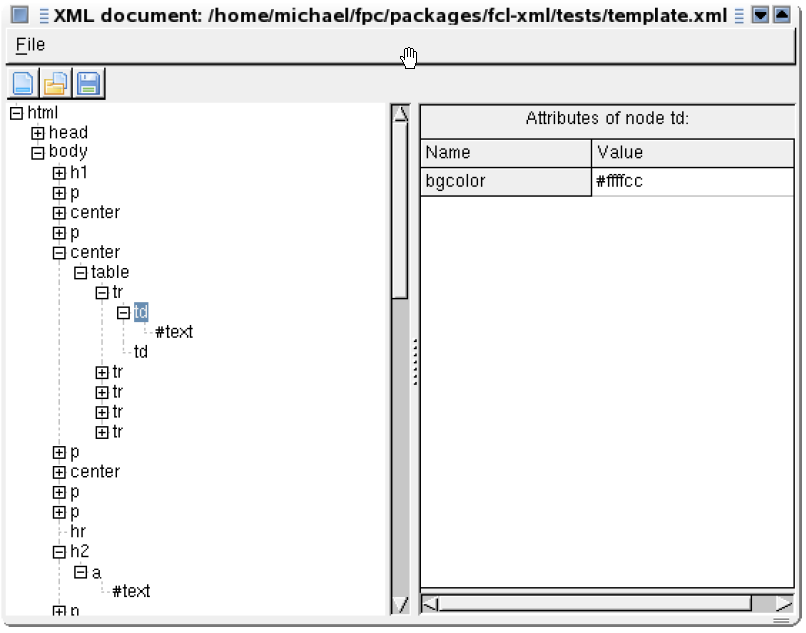
\includegraphics{D:/Archive/github/translations/webdata_lazarus_fpc/webdata_rus.assets/fig_1_xml_viewer_app.png}\tabularnewline
\bottomrule
\end{longtable}

Чтобы продемонстрировать возможности манипулирования моделью DOM, будет
добавлен некоторый код для добавления текстовых узлов или узлов
элементов в дерево DOM. Для этого создается новый элемент меню и кнопка
на панели инструментов, которая создаст новый элемент относительно
текущего элемента. Код, выполняемый пунктом меню, будет выглядеть
следующим образом:

\begin{Shaded}
\begin{Highlighting}[]
\KeywordTok{procedure}\NormalTok{ TMainForm.ANewElementExecute(Sender: TObject);}
\KeywordTok{var}
\NormalTok{  P,N: TDomNode;}
\NormalTok{  PT: TTreeNode;}
\KeywordTok{begin}
\NormalTok{  P:= }\KeywordTok{nil}\NormalTok{;}
\NormalTok{  PT:= TVXML.Selected;}
  \KeywordTok{if}\NormalTok{ Assigned(PT) }\KeywordTok{then}
\NormalTok{    P:= TDOMNode(PT.Data)}
  \KeywordTok{else}
\NormalTok{    P:= FXML;}

\NormalTok{  N:= NewElement(P,PT);}

  \KeywordTok{if}\NormalTok{ (N \textless{}\textgreater{} }\KeywordTok{nil}\NormalTok{) }\KeywordTok{then}
  \KeywordTok{begin}
\NormalTok{    ClearNodeData;}
\NormalTok{    ShowNodeData(N);}
  \KeywordTok{end}\NormalTok{;}
\KeywordTok{end}\NormalTok{;}
\end{Highlighting}
\end{Shaded}

Сначала определяется текущий dom-узел. Если ничего не найдено (например,
когда документ пуст), то сам документ устанавливается как текущий узел
dom (TXMLDocument также является потомком \texttt{TDOMNode}). Вызов
\texttt{NewElement} выполняет реальную работу. Если он возвращает узел,
то отображаются данные узла.

Настоящая работа происходит в функции \texttt{NewElement}:

\begin{Shaded}
\begin{Highlighting}[]
\KeywordTok{function}\NormalTok{ TMainForm.NewElement(P: TDomNode; PT: TTreeNode): TDomNode;}
\KeywordTok{var}
\NormalTok{  N,NN: TDomNode;}
\NormalTok{  NT: }\DataTypeTok{integer}\NormalTok{;}
\NormalTok{  NL: TNodeLocation;}
\NormalTok{  S: }\DataTypeTok{String}\NormalTok{;}
\NormalTok{  TN: TTreeNode;}
\KeywordTok{begin}
\NormalTok{  Result:= }\KeywordTok{nil}\NormalTok{;}
  \KeywordTok{with}\NormalTok{ TNewNodeForm.Create(}\KeywordTok{Self}\NormalTok{) }\KeywordTok{do}
  \KeywordTok{try}
\NormalTok{    HaveParent:= P.ParentNode \textless{}\textgreater{} }\KeywordTok{nil}\NormalTok{;}
    \KeywordTok{if}\NormalTok{ (ShowModal \textless{}\textgreater{} mrOK) }\KeywordTok{then} \KeywordTok{Exit}\NormalTok{;}

\NormalTok{    NT:= NodeType;}
\NormalTok{    NL:= NodeLocation;}
\NormalTok{    S:= NodeText;}
  \KeywordTok{finally}
\NormalTok{    Free;}
  \KeywordTok{end}\NormalTok{;}
\KeywordTok{end}\NormalTok{;}
\end{Highlighting}
\end{Shaded}

Эта первая часть только собирает данные: в ней отображается диалоговое
окно (\texttt{TNewNodeForm}, его детали не имеют отношения к
обсуждению), в котором спрашивается, какой тип узла должен быть создан,
где он должен быть создан и какой текст он должен содержать. С этими
данными фактическая работа сделана. Сначала создается узел. Для этого
используется вызов \texttt{TXMLDocument}:

\begin{Shaded}
\begin{Highlighting}[]
\KeywordTok{case}\NormalTok{ NT }\KeywordTok{of}
\NormalTok{ ELEMENT\_NODE: N:= FXML.CreateElement(S);}
\NormalTok{    TEXT\_NODE:}
          \KeywordTok{begin}
\NormalTok{            N:= FXML.CreateTextNode(S);}
\NormalTok{            NL:= nlLastChild;}
          \KeywordTok{end}\NormalTok{;}
\KeywordTok{end}\NormalTok{;}

\KeywordTok{if}\NormalTok{ (P.NodeType = TEXT\_NODE) }\KeywordTok{then}\NormalTok{ nl:= nlReplaceCurrent;}
\end{Highlighting}
\end{Shaded}

Когда узел создается, местоположение узла используется для определения
того, где в дереве DOM должен быть вставлен новый узел. Возможны не все
комбинации: текстовый узел всегда является листовым узлом (то есть он
всегда должен быть единственным дочерним узлом от своего родителя).
Некоторые проверки сделаны для этого.

После этого узел вставляется в дерево DOM, и одновременно обновляется
древовидная структура:

\begin{Shaded}
\begin{Highlighting}[]
\KeywordTok{case}\NormalTok{ NL }\KeywordTok{of}
\NormalTok{     nlFirstChild:}
                  \KeywordTok{begin}
\NormalTok{                    NN:= P.FirstChild;}
                    \KeywordTok{if}\NormalTok{ (NN \textless{}\textgreater{} }\KeywordTok{nil}\NormalTok{) }\KeywordTok{then}
\NormalTok{                      P.InsertBefore(N,NN)}
                    \KeywordTok{else}
\NormalTok{                      P.AppendChild(N);}

\NormalTok{                    TN:= TVXML.Items.AddChildFirst(PT,N.NodeName);}
                  \KeywordTok{end}\NormalTok{;}
\NormalTok{      nlLastChild:}
                  \KeywordTok{begin}
\NormalTok{                    P.AppendChild(N);}
\NormalTok{                    TN:= TVXML.Items.AddChild(PT,N.NodeName);}
                  \KeywordTok{end}\NormalTok{;}
\NormalTok{  nlBeforeCurrent:}
                  \KeywordTok{begin}
\NormalTok{                    P.ParentNode.InsertBefore(N,P);}
\NormalTok{                    TN:= TVXML.Items.Insert(PT,N.NodeName);}
                  \KeywordTok{end}\NormalTok{;}
\NormalTok{ nlReplaceCurrent:}
                  \KeywordTok{begin}
\NormalTok{                    P.ParentNode.ReplaceChild(N,P);}
\NormalTok{                    PT.}\DataTypeTok{Text}\NormalTok{:= N.NodeName;}
\NormalTok{                    TN:= PT;}
                  \KeywordTok{end}\NormalTok{;}
  \KeywordTok{end}\NormalTok{;}\CommentTok{\{case..of\}}

\NormalTok{  TN.Data:= N;}
\NormalTok{  TVXML.Selected:= TN;}
\NormalTok{  Result:= N;}
\end{Highlighting}
\end{Shaded}

Код для изменения свойств узла (текста или атрибутов) оставлен на
усмотрение заинтересованного читателя.

Для навигации и поиска узлов в дереве документов XML W3 создал
спецификацию \texttt{XPath}\footnote{https://www.w3.org/TR/xpath20}.
Модуль \texttt{XPath}, поставляемый с Free Pascal, содержит реализацию
этой спецификации. Основной функцией этого модуля является вызов
\texttt{EvaluateXPathExpression}:

\begin{Shaded}
\begin{Highlighting}[]
\KeywordTok{function}\NormalTok{ EvaluateXPathExpression(}\KeywordTok{const}\NormalTok{ AExpressionString: DOMString; AContextNode: TDOMNode): TXPathVariable;}
\end{Highlighting}
\end{Shaded}

Эта функция оценивает выражение \texttt{XPath}, начиная
с\texttt{AContextNode}, и возвращает результат в виде экземпляра
\texttt{TXPathVariable}. Класс \texttt{TXPathVariable} является базовым
классом для всех результатов \texttt{XPath}, есть много потомков этого
класса, каждый из которых представляет возможный результат запроса
(который может быть числом, текстом, набором узлов и т. Д.)

Полное обсуждение \texttt{XPath} выходит за рамки этой статьи, но будет
дан небольшой пример, чтобы показать, как его можно использовать для
быстрого поиска узла в дереве: для этого пункт меню
\texttt{Go\ to\ node} («Перейти к узлу») сделано под меню \texttt{Edit}
(«Правка»). При нажатии выполняется следующий код:

\begin{Shaded}
\begin{Highlighting}[]
\KeywordTok{procedure}\NormalTok{ TMainForm.AGotoExecute(Sender: TObject);}
\KeywordTok{var}
\NormalTok{  S: }\DataTypeTok{String}\NormalTok{;}
\NormalTok{  V: TXPathVariable;}
\NormalTok{  N: TNodeSet;}
\KeywordTok{begin}
  \KeywordTok{if}\NormalTok{ Assigned(FXML.DocumentElement) }\KeywordTok{then}
\NormalTok{    S:=}\StringTok{\textquotesingle{}/\textquotesingle{}}\NormalTok{ + FXML.DocumentElement.NodeName}
  \KeywordTok{else}
\NormalTok{    S:= }\StringTok{\textquotesingle{}\textquotesingle{}}\NormalTok{;}

  \KeywordTok{if}\NormalTok{ InputQuery(SGoto,SSpecifyPath,S) }\KeywordTok{then}
  \KeywordTok{begin}
\NormalTok{    V:= EvaluateXPathExpression(S,FXML);}

    \KeywordTok{try}
    \KeywordTok{if} \KeywordTok{not}\NormalTok{ (V }\KeywordTok{is}\NormalTok{ TXPathNodeSetVariable) }\KeywordTok{then}
\NormalTok{      ShowMessage(SErrNotaNode)}
    \KeywordTok{else}
      \KeywordTok{begin}
\NormalTok{      N:= V.AsNodeSet;}

      \KeywordTok{if}\NormalTok{ (N.Count \textless{}\textgreater{} }\DecValTok{1}\NormalTok{) }\KeywordTok{then}
\NormalTok{        ShowMessage(SErrSingleNode)}
      \KeywordTok{else}
\NormalTok{        GotoNode(TDOMNode(N.Items[}\DecValTok{0}\NormalTok{]));}
      \KeywordTok{end}\NormalTok{;}
    \KeywordTok{finally}
\NormalTok{      V.Free;}
    \KeywordTok{end}\NormalTok{;}
  \KeywordTok{end}\NormalTok{;}
\KeywordTok{end}\NormalTok{;}
\end{Highlighting}
\end{Shaded}

Сначала определяется местоположение корневого узла для операции поиска
(это может быть расширено, например, для поиска, начинающегося на
текущем узле). Это значение используется для запроса пользователя о
поиске пути. Затем путь передается вызову
\texttt{EvaluateXPathExpression} вместе с документом XML в качестве
корня операции поиска. Если результат имеет тип
\texttt{TXPathNodeSetVariable}, то оценка выражения \texttt{XPath}
привела к одному или нескольким узлам DOM. Набор узлов результата
возвращается как свойство \texttt{AsNodeSet}, которое представляет собой
\texttt{TList}. Если список содержит один узел, он передается в вызов
\texttt{GotoNode}, который отображает узел в дереве.

Средство просмотра XML можно использовать для проверки, например, файла
с информацией о проекте Lazarus (\texttt{.lpi}) в формате XML. Следующий
путь:

\begin{verbatim}
/CONFIG/ProjectOptions/Units/Unit1/Filename
\end{verbatim}

Развернется узел, содержащий имя файла первого модуля в проекте.
Выражение \texttt{XPATH}

\begin{verbatim}
/CONFIG/ProjectOptions/Units/*/Filename
\end{verbatim}

Результатом будет набор узлов с именами всех модулей в проекте.
Поскольку в дереве может отображаться только один узел, это может
привести к сообщению об ошибке.

\hypertarget{header-n2529}{%
\subsection{JSON: структуры данных.}\label{header-n2529}}

Спецификация \texttt{JSON} (JavaScript Object Notation)\footnote{https://www.json.org/json-ru.html
  (в оригинальном документе https://www.json.org/json-en.html)} гораздо
проще, чем спецификации XML: она помещается на одном листе бумаги.
Спецификация ориентирована на использование в браузерах: действительно,
JSON был задуман для быстрой отправки структурированных данных в браузер
без необходимости сложных структур DOM и парсеров. Вместо этого
встроенный механизм \texttt{JavaScript} используется для преобразования
данных \texttt{JSON} в объект \texttt{JavaScript}, готовый для
использования в браузере. Эта простота и скорость, вероятно, объясняют
его быстрое принятие программистами веб-приложений - особенно в не
корпоративных условиях.

Ниже приведен пример данных \texttt{JSON}:

\begin{Shaded}
\begin{Highlighting}[]
\FunctionTok{\{}
 \DataTypeTok{"addressbook"}\FunctionTok{:} \FunctionTok{\{}\DataTypeTok{"name"}\FunctionTok{:} \StringTok{"Mary Lebow"}\FunctionTok{,} 
     \DataTypeTok{"address"}\FunctionTok{:} \FunctionTok{\{}\DataTypeTok{"street"}\FunctionTok{:} \StringTok{"5 Main Street"}\FunctionTok{,}  \DataTypeTok{"city"}\FunctionTok{:} \StringTok{"San Diego, CA"}\FunctionTok{,} \DataTypeTok{"zip"}\FunctionTok{:} \DecValTok{91912} \FunctionTok{\},} 
\DataTypeTok{"phoneNumbers"}\FunctionTok{:} \OtherTok{[}\StringTok{"619 332{-}3452"}\OtherTok{,}\StringTok{"664 223{-}4667"}\OtherTok{]}\FunctionTok{\}} 
\FunctionTok{\}}
\end{Highlighting}
\end{Shaded}

Который в XML будет представлен, например, как:

\begin{Shaded}
\begin{Highlighting}[]
\KeywordTok{\textless{}addressbook\textgreater{}}
 \KeywordTok{\textless{}name\textgreater{}}\NormalTok{Mary Lebow}\KeywordTok{\textless{}/name\textgreater{}}
 \KeywordTok{\textless{}address\textgreater{}\textless{}street\textgreater{}}\NormalTok{5 Main Street}\KeywordTok{\textless{}/street\textgreater{}}
          \KeywordTok{\textless{}city}\OtherTok{ zip=}\StringTok{"91912"}\KeywordTok{\textgreater{}}\NormalTok{San Diego, CA}\KeywordTok{\textless{}/city\textgreater{}}
          \KeywordTok{\textless{}phoneNumbers\textgreater{}\textless{}phone\textgreater{}}\NormalTok{619 332{-}3452}\KeywordTok{\textless{}/phone\textgreater{}}
                        \KeywordTok{\textless{}phone\textgreater{}}\NormalTok{664 223{-}4667}\KeywordTok{\textless{}/phone\textgreater{}}
          \KeywordTok{\textless{}/phoneNumbers\textgreater{}}
 \KeywordTok{\textless{}/address\textgreater{}}
\KeywordTok{\textless{}/addressbook\textgreater{}}
\end{Highlighting}
\end{Shaded}

(пример взят
\href{https://www.oracle.com/technical-resources/articles/enterprise-architecture/introduction-json.html}{отсюда}(\emph{прим.перев.:}
в оригинальном документе
\href{https://www.json.org/json-en.html}{отсюда})).

Спецификация \texttt{JSON} описывает только текстовый формат данных, но
не дает никаких спецификаций о том, как обрабатывать данные. Поскольку
это \texttt{JavaScript}, в этом нет необходимости, так как данные
преобразуются непосредственно в объекты и массивы \texttt{JavaScript}.
Для других языков, таких как \texttt{Object\ Pascal}, спецификация
отсутствует. Следовательно, реализация, предоставляемая Free Pascal,
является не реализацией стандарта, а реализацией, которая, как полагают,
проста для быстрого создания и проверки данных. Модуль \texttt{fpjson}
содержит реализацию \texttt{JSON} для Free Pascal. Базовая структура
объектов для реализации \texttt{JSON} показана на рисунке 2.

\begin{longtable}[]{@{}l@{}}
\toprule
Рисунок 2: Структура данных JSON в fpjson\tabularnewline
\midrule
\endhead
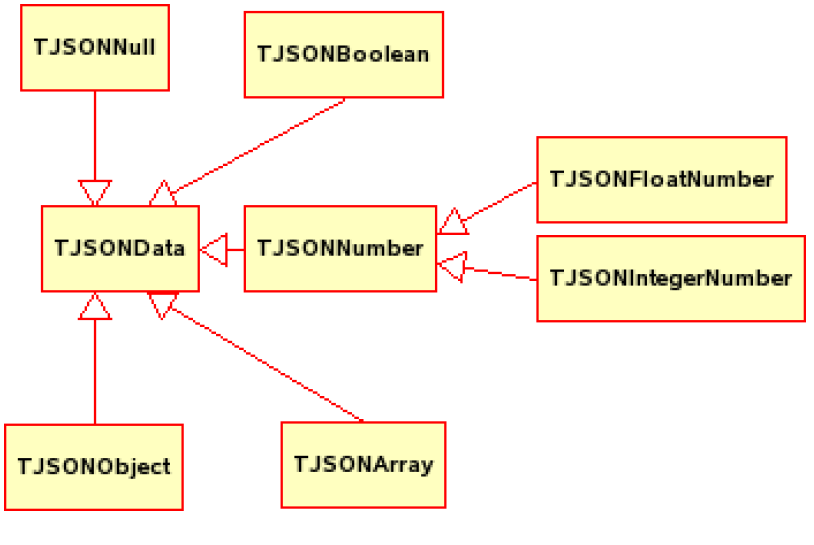
\includegraphics{D:/Archive/github/translations/webdata_lazarus_fpc/webdata_rus.assets/fig_2_fpjson_data_struct.png}\tabularnewline
\bottomrule
\end{longtable}

Базовый класс - \texttt{TJSONData}. Он имеет следующие свойства:

\begin{itemize}
\item
  \texttt{JSONType} - перечислимый, который содержит тип данных для
  этого объекта.
\item
  \texttt{IsNull} равен \texttt{True}, если значение равно
  \texttt{NULL}.
\item
  \texttt{AsBoolean} - значение данных как логическое значение.
\item
  \texttt{AsInteger} - значение данных в виде целого числа.
\item
  \texttt{AsFloat} - значение данных как \texttt{double} или
  \texttt{extended}.
\item
  \texttt{AsString} - значение данных в виде строки.
\item
  \texttt{Count} - количество элементов, содержащихся в этом элементе
  данных. Очевидно, это будет только ненулевое значение для объектов и
  массивов.
\item
  \texttt{Items} - это свойство массива предоставляет доступ к
  элементам, содержащимся в этом элементе данных. Каждый элемент
  является потомком \texttt{TJSONData}. Обратите внимание, что элементы
  могут быть разных типов: массив может содержать смесь целых чисел,
  строк, нулевых значений.
\item
  \texttt{AsJSON} возвращает содержимое значения (и его вложенных
  значений, если это массив или объект) в виде строки \texttt{JSON}.
\end{itemize}

Потомки этого класса - по одному на тип данных \texttt{JSON}, как видно
на рис.2, хранят фактические данные. Их конструктор принимает значение
данных в качестве параметра. Чтобы создать строковое значение
\texttt{JSON}, нужно выполнить следующий код:

\begin{Shaded}
\begin{Highlighting}[]
\NormalTok{J:=TJSONString.Create(}\StringTok{\textquotesingle{}A string\textquotesingle{}}\NormalTok{);}
\end{Highlighting}
\end{Shaded}

Конструкторы \texttt{TJSONObject} и \texttt{TJSONArray} опционально
принимают массив констант и заполняют объект или массив значениями в
массиве.

\begin{Shaded}
\begin{Highlighting}[]
\NormalTok{Ja:=TJSONArray.Create([}\KeywordTok{Nil}\NormalTok{, }\KeywordTok{True}\NormalTok{, }\DecValTok{1}\NormalTok{, }\DecValTok{2.3}\NormalTok{, }\StringTok{\textquotesingle{}String\textquotesingle{}}\NormalTok{]); }
\NormalTok{Jo:=TJSONObject.Create([}\StringTok{\textquotesingle{}a\textquotesingle{}}\NormalTok{,}\DecValTok{1}\NormalTok{,}\StringTok{\textquotesingle{}b\textquotesingle{}}\NormalTok{,ja]);}
\end{Highlighting}
\end{Shaded}

Обратите внимание, что конструктору \texttt{TJSONObject} нужны аргументы
в парах: \texttt{имя} (всегда строка) и \texttt{значение} (почти любой
допустимый базовый тип \texttt{JSON}). Из примера также видно, что
массив также может содержать другие экземпляры \texttt{TJSONData}.

Тип массива \texttt{TJSONArray} также можно манипулировать с помощью
простых вызовов \texttt{add}:

\begin{Shaded}
\begin{Highlighting}[]
\KeywordTok{function}\NormalTok{ Add(Item: TJSONData): }\DataTypeTok{Integer}\NormalTok{;}
\KeywordTok{function}\NormalTok{ Add(I: }\DataTypeTok{Integer}\NormalTok{): }\DataTypeTok{Integer}\NormalTok{;}
\KeywordTok{function}\NormalTok{ Add(S: }\DataTypeTok{String}\NormalTok{): }\DataTypeTok{Integer}\NormalTok{;}
\KeywordTok{function}\NormalTok{ Add: }\DataTypeTok{Integer}\NormalTok{;}
\KeywordTok{function}\NormalTok{ Add(F: TJSONFloat): }\DataTypeTok{Integer}\NormalTok{;}
\KeywordTok{function}\NormalTok{ Add(B: }\DataTypeTok{Boolean}\NormalTok{): }\DataTypeTok{Integer}\NormalTok{;}
\KeywordTok{function}\NormalTok{ Add(AnArray: TJSONArray): }\DataTypeTok{Integer}\NormalTok{;}
\KeywordTok{function}\NormalTok{ Add(AnObject: TJSONObject): }\DataTypeTok{Integer}\NormalTok{;}
\KeywordTok{procedure}\NormalTok{ Delete(Index: }\DataTypeTok{Integer}\NormalTok{);}
\KeywordTok{procedure}\NormalTok{ Remove(Item: TJSONData);}
\end{Highlighting}
\end{Shaded}

Вызовы \texttt{Add} заботятся о создании правильного потомка
\texttt{TJSONData}. Значение вызовов \texttt{Delete} и \texttt{Remove}
должно быть ясным. Аналогичные вызовы существуют для класса
\texttt{TJSONObject}, но они принимают дополнительный аргумент: имя
добавляемого элемента. Вооружившись всеми этими вызовами, приведенные
выше данные \texttt{JSON} могут быть сформированы следующим образом:

\begin{Shaded}
\begin{Highlighting}[]
\KeywordTok{procedure}\NormalTok{ TestLong;}
\KeywordTok{var}
\NormalTok{  JAB,J,JA: TJSONObject;}
\NormalTok{  JT: TJSONArray;}
\KeywordTok{begin}
\NormalTok{  JA:=TJSonObject.Create;}
\NormalTok{  JA.Add(}\StringTok{\textquotesingle{}street\textquotesingle{}}\NormalTok{,}\StringTok{\textquotesingle{}5 Main Street\textquotesingle{}}\NormalTok{);}
\NormalTok{  JA.Add(}\StringTok{\textquotesingle{}City\textquotesingle{}}\NormalTok{,}\StringTok{\textquotesingle{}San Diego, CA\textquotesingle{}}\NormalTok{);}
\NormalTok{  JA.Add(}\StringTok{\textquotesingle{}Zip\textquotesingle{}}\NormalTok{,}\DecValTok{91912}\NormalTok{);}
\NormalTok{  JT:=TJSonArray.Create;}
\NormalTok{  JT.Add(}\StringTok{\textquotesingle{}619 332{-}3452\textquotesingle{}}\NormalTok{);}
\NormalTok{  JT.Add(}\StringTok{\textquotesingle{}664 223{-}4667\textquotesingle{}}\NormalTok{);}

\NormalTok{  J:= TJSONObject.Create;}
\NormalTok{  J.Add(}\StringTok{\textquotesingle{}name\textquotesingle{}}\NormalTok{,}\StringTok{\textquotesingle{}Mary Lebow\textquotesingle{}}\NormalTok{);}
\NormalTok{  J.Add(}\StringTok{\textquotesingle{}address\textquotesingle{}}\NormalTok{,JA);}
\NormalTok{  J.Add(}\StringTok{\textquotesingle{}phonenumbers\textquotesingle{}}\NormalTok{,JT);}

\NormalTok{  JAB:= TJSONObject.Create;}
\NormalTok{  JAB.Add(}\StringTok{\textquotesingle{}addressbook\textquotesingle{}}\NormalTok{,J);}
\NormalTok{  Writeln(JAB.AsJSON);}
\NormalTok{  JAB.Free;}
\KeywordTok{end}\NormalTok{;}
\end{Highlighting}
\end{Shaded}

Или короче:

\begin{Shaded}
\begin{Highlighting}[]
\KeywordTok{procedure}\NormalTok{ TestShort;}
\KeywordTok{var}
\NormalTok{  JAB,J,JA: TJSONObject;}
\NormalTok{  JT: TJSONArray;}
\KeywordTok{begin}
\NormalTok{  JA:= TJSonObject.Create([}\StringTok{\textquotesingle{}street\textquotesingle{}}\NormalTok{,}\StringTok{\textquotesingle{}5 Main Street\textquotesingle{}}\NormalTok{,}
                          \StringTok{\textquotesingle{}City\textquotesingle{}}\NormalTok{,}\StringTok{\textquotesingle{}San Diego, CA\textquotesingle{}}\NormalTok{,}
                          \StringTok{\textquotesingle{}Zip\textquotesingle{}}\NormalTok{,}\DecValTok{91912}\NormalTok{]);}
\NormalTok{  JT:= TJSonArray.Create([}\StringTok{\textquotesingle{}619 332{-}3452\textquotesingle{}}\NormalTok{,}\StringTok{\textquotesingle{}664 223{-}4667\textquotesingle{}}\NormalTok{]);}
\NormalTok{  J:= TJSONObject.Create([}\StringTok{\textquotesingle{}name\textquotesingle{}}\NormalTok{,}\StringTok{\textquotesingle{}Mary Lebow\textquotesingle{}}\NormalTok{,}
                          \StringTok{\textquotesingle{}address\textquotesingle{}}\NormalTok{,JA,}\StringTok{\textquotesingle{}phonenumbers\textquotesingle{}}\NormalTok{,JT]);}
\NormalTok{  JAB:= TJSONObject.Create([}\StringTok{\textquotesingle{}addressbook\textquotesingle{}}\NormalTok{,J]);}
\NormalTok{  Writeln(JAB.AsJSON);}
\NormalTok{  JAB.Free;}
\KeywordTok{end}\NormalTok{;}
\end{Highlighting}
\end{Shaded}

Это можно сделать еще короче без вспомогательных переменных, но тогда
код становится нечитаемым. Быстрая проверка выходных данных убедит
любого, что выходные данные одинаковы в обоих случаях и соответствуют
приведенному выше образцу \texttt{JSON}.

Обратите внимание, что последнее процедура:

\begin{Shaded}
\begin{Highlighting}[]
\NormalTok{JAB.Free}
\end{Highlighting}
\end{Shaded}

освобождает также все другие созданные объекты: \texttt{TSJONArray} или
\texttt{TJSONObject} владеет содержащимися в нем элементами.

Запись \texttt{TJSONFile} чрезвычайно проста, как видно из тестового
кода выше: метод \texttt{AsJSON} возвращает строку, описывающую данные
\texttt{JSON} в допустимом формате \texttt{JSON}. Единственное, что
нужно сделать, это записать ее в поток.

Для чтения данных \texttt{JSON} модуль \texttt{jsonparser} содержит
класс \texttt{TJSONParser}. Он содержит один вызов: \texttt{Parse},
который возвращает экземпляр \texttt{TJSONData}, соответствующий данным
\texttt{JSON}, которые он считывает из строки или потока, который может
быть указан в конструкторе класса.

\hypertarget{header-n2580}{%
\subsection{Просмотрщик данных JSON.}\label{header-n2580}}

Подобно средству просмотра \texttt{XML}, средство просмотра данных
\texttt{JSON} может быть закодировано. Общий код и логика программы
такие же, как у программы просмотра \texttt{XML}. Только некоторые
подробные процедуры изменены.

Например, вызов для чтения данных \texttt{JSON} из файла выглядит
следующим образом:

\begin{Shaded}
\begin{Highlighting}[]
\KeywordTok{procedure}\NormalTok{ TMainForm.OpenFile(AFileName : }\DataTypeTok{String}\NormalTok{);}
\KeywordTok{var}
\NormalTok{  J: TJSONData;}
\NormalTok{  F: TFileStream;}
\KeywordTok{begin}
\NormalTok{  F:= TFileStream.Create(AFileName,fmOpenRead);}
  \KeywordTok{try}
    \KeywordTok{with}\NormalTok{ TJSONParser.Create(F) }\KeywordTok{do}
    \KeywordTok{try}
\NormalTok{      J:= Parse;}
    \KeywordTok{finally}
\NormalTok{      Free;}
    \KeywordTok{end}\NormalTok{;}
  \KeywordTok{finally}
\NormalTok{    F.FRee;}
  \KeywordTok{end}\NormalTok{;}

  \KeywordTok{if}\NormalTok{ J.JSONType \textless{}\textgreater{} jtObject }\KeywordTok{then}
    \KeywordTok{Raise}\NormalTok{ Exception.Create(SErrNoJSONObject);}

  \KeywordTok{if}\NormalTok{ Assigned(FJSON) }\KeywordTok{then}\NormalTok{ FreeAndNil(FJSON);}

\NormalTok{  FJSON:= J }\KeywordTok{as}\NormalTok{ TJSONObject;}
\NormalTok{  SetFileName(AFileName);}
\NormalTok{  ShowObject(FJSON);}
\KeywordTok{end}\NormalTok{;}
\end{Highlighting}
\end{Shaded}

Переменная \texttt{FXML}, существовавшая в средстве просмотра
\texttt{XML}, была заменена на переменную \texttt{FJSON} типа
\texttt{TJSONObject}. Обратите внимание на проверку, является ли
возвращаемый \texttt{TJSONParser} объект \texttt{TJSONObject}.
Анализатор также может возвращать простой тип, и он не может
отображаться в виде дерева.

Вызов для построения дерева очень похож на его XML-сережку - это простой
рекурсивный алгоритм:

\begin{Shaded}
\begin{Highlighting}[]
\KeywordTok{function}\NormalTok{ TMainForm.ShowNode(AParent: TTreeNode; AName: }\DataTypeTok{String}\NormalTok{; J: TJSONData): TTreeNode;}
\KeywordTok{var}
\NormalTok{  O: TJSONObject;}
\NormalTok{  I: }\DataTypeTok{Integer}\NormalTok{;}
\KeywordTok{begin}
  \KeywordTok{if} \KeywordTok{not}\NormalTok{ (J.JSONType }\KeywordTok{in}\NormalTok{ [jtArray,jtObject]) }\KeywordTok{then}
\NormalTok{    AName:= AName+ }\StringTok{\textquotesingle{} : \textquotesingle{}}\NormalTok{ + J.AsJSON;}
\NormalTok{  Result:= TVJSON.Items.AddChild(AParent,AName);}
\NormalTok{  Result.Data:= J;}

  \KeywordTok{if}\NormalTok{ (J.Count \textless{}\textgreater{} }\DecValTok{0}\NormalTok{) }\KeywordTok{then}
  \KeywordTok{begin}
    \KeywordTok{if}\NormalTok{ (j }\KeywordTok{is}\NormalTok{ TJSONObject) }\KeywordTok{then}
      \KeywordTok{begin}
\NormalTok{        O:= J }\KeywordTok{as}\NormalTok{ TJSONObject;}
        \KeywordTok{for}\NormalTok{ I:= }\DecValTok{0} \KeywordTok{to}\NormalTok{ O.Count}\DecValTok{{-}1} \KeywordTok{do}
\NormalTok{        ShowNode(Result,O.Names[i],O.Items[i]);}
      \KeywordTok{end}
    \KeywordTok{else}
      \KeywordTok{if}\NormalTok{ (j }\KeywordTok{is}\NormalTok{ TJSONArray) }\KeywordTok{then}
      \KeywordTok{begin}
        \KeywordTok{for}\NormalTok{ I:= }\DecValTok{0} \KeywordTok{to}\NormalTok{ J.Count}\DecValTok{{-}1} \KeywordTok{do}
\NormalTok{        ShowNode(Result,IntToStr(I),J.Items[i]);}
      \KeywordTok{end}\NormalTok{;}
  \KeywordTok{end}\NormalTok{;}
\KeywordTok{end}
\end{Highlighting}
\end{Shaded}

Обратите внимание, что каждый узел отображается со своим добавленным
значением, если это простой тип. Элементы массива отображаются с их
индексом в качестве имени узла, а элементы объекта отображаются с их
именем.

Отображение данных узла на панели сведений происходит так же, как и для
средства просмотра \texttt{XML}. Код ниже показывает, как это делается
для массива \texttt{JSON}:

\begin{Shaded}
\begin{Highlighting}[]
\KeywordTok{procedure}\NormalTok{ TMainForm.ShowArrayData(A : TJSONArray);}
\KeywordTok{var}
\NormalTok{  G: TStringGrid;}
\NormalTok{  I: }\DataTypeTok{Integer}\NormalTok{;}
\NormalTok{  J: TJSONData;}
\KeywordTok{begin}
\NormalTok{  DataTopLabel(SArrayData);}
\NormalTok{  G:= TStringGrid.Create(}\KeywordTok{Self}\NormalTok{);}
\NormalTok{  G.Parent:= PDetails;}
\NormalTok{  G.Align:= alClient;}
\NormalTok{  G.FixedCols:= }\DecValTok{0}\NormalTok{;}
\NormalTok{  G.RowCount:= }\DecValTok{2}\NormalTok{;}
\NormalTok{  G.ColCount:= }\DecValTok{1}\NormalTok{;}
\NormalTok{  G.Cells[}\DecValTok{0}\NormalTok{,}\DecValTok{0}\NormalTok{]:= SElementValue;}
\NormalTok{  G.RowCount:= }\DecValTok{1}\NormalTok{ + A.Count;}
\NormalTok{  G.Options:= G.Options + [goColSizing];}

  \KeywordTok{if}\NormalTok{ (G.RowCount\textgreater{}}\DecValTok{0}\NormalTok{) }\KeywordTok{then}
\NormalTok{    G.FixedRows:=}\DecValTok{1}
  \KeywordTok{else}
\NormalTok{    G.FixedRows:=}\DecValTok{0}\NormalTok{;}

  \KeywordTok{for}\NormalTok{ I:= }\DecValTok{1} \KeywordTok{to}\NormalTok{ A.Count }\KeywordTok{do}
  \KeywordTok{begin}
\NormalTok{    J:= A.Items[i}\DecValTok{{-}1}\NormalTok{];}
    \KeywordTok{if}\NormalTok{ (J.JSONType }\KeywordTok{in}\NormalTok{ [jtArray,jtObject,jtNull]) }\KeywordTok{then}
\NormalTok{      G.Cells[}\DecValTok{0}\NormalTok{,I]:= J.AsJSON}
    \KeywordTok{else}
\NormalTok{      G.Cells[}\DecValTok{0}\NormalTok{,I]:= J.AsString;}
  \KeywordTok{end}\NormalTok{;}
\KeywordTok{end}\NormalTok{;}
\end{Highlighting}
\end{Shaded}

Как видно, массив отображается в виде сетки с одним столбцом: каждый
элемент массива находится в строке. Если это простой тип (булево, число
или строка), то отображается значение. Для сложных типов отображается
представление \texttt{JSON}.

Для отображения объектов на панели сведений используется та же логика,
но сетка содержит 2 столбца: первый содержит имя каждого элемента в
объекте, второй отображает значение.

Наконец, что не менее важно, новое значение может быть добавлено в
дерево. Метод \texttt{NewElement} основной формы позаботится об этом:

\begin{Shaded}
\begin{Highlighting}[]
\KeywordTok{function}\NormalTok{ TMainForm.NewElement(P: TJSONData; PT: TTreeNode): TJSONData;}
\KeywordTok{var}
\NormalTok{  NT: TJSonType;}
\NormalTok{  EN,EV: }\DataTypeTok{String}\NormalTok{;}
\NormalTok{  TN: TTreeNode;}
\NormalTok{  I: }\DataTypeTok{Integer}\NormalTok{;}
\KeywordTok{begin}
\NormalTok{  Result:= }\KeywordTok{nil}\NormalTok{;}

  \KeywordTok{with}\NormalTok{ TNewElementForm.Create(}\KeywordTok{Self}\NormalTok{) }\KeywordTok{do}
  \KeywordTok{try}
\NormalTok{    NeedName:= P }\KeywordTok{is}\NormalTok{ TJSONObject;}
    \KeywordTok{if}\NormalTok{ (ShowModal \textless{}\textgreater{} mrOK) }\KeywordTok{then} \KeywordTok{Exit}\NormalTok{;}
\NormalTok{    NT:= DataType;}
\NormalTok{    EN:= ElementName;}
\NormalTok{    EV:= ElementValue;}
  \KeywordTok{finally}
\NormalTok{    Free;}
  \KeywordTok{end}\NormalTok{;}
\KeywordTok{end}\NormalTok{;}
\end{Highlighting}
\end{Shaded}

В этой первой части отображается диалоговое окно для запроса у
пользователя значения, которое следует добавить. Обратите внимание, что
свойство \texttt{NeedName} \texttt{TElementForm} решает, должен ли
пользователь вводить имя для значения или нет: в случае добавления
нового значения к объекту новое значение также должно получить имя.

После того, как все данные были получены от пользователя, новое значение
может быть действительно создано и добавлено в родительский объект.
Поскольку модуль \texttt{fpjson} содержит 2 типа для числового значения
\texttt{JSON}, требуется некоторая логика, чтобы увидеть, следует ли
создавать число с плавающей запятой или целое число:

\begin{Shaded}
\begin{Highlighting}[]
\KeywordTok{case}\NormalTok{ NT }\KeywordTok{of}
\NormalTok{    jtNumber: }\KeywordTok{if}\NormalTok{ TryStrToInt(EV,I) }\KeywordTok{then}
\NormalTok{                Result:= TJSONIntegerNumber.Create(i)}
              \KeywordTok{else}
\NormalTok{                Result:= TJSONFloatNumber.Create(StrToFloat(EV));}
\NormalTok{      jtNull: Result:= TJSONNull.Create;}
\NormalTok{    jtString: Result:= TJSONString.Create(EV);}
\NormalTok{   jtBoolean: Result:= TJSONBoolean.Create(StrToBool(EV));}
\NormalTok{     jtArray: Result:= TJSONArray.Create;}
\NormalTok{    jtObject: Result:= TJSONObject.Create;}
    \KeywordTok{end}\NormalTok{;}

    \KeywordTok{if}\NormalTok{ P }\KeywordTok{is}\NormalTok{ TJSONObject }\KeywordTok{then}
\NormalTok{      (P }\KeywordTok{as}\NormalTok{ TJSONObject).Add(EN,Result)}
    \KeywordTok{else} \KeywordTok{if}\NormalTok{ (P }\KeywordTok{is}\NormalTok{ TJSONArray) }\KeywordTok{then}
\NormalTok{          (P }\KeywordTok{as}\NormalTok{ TJSONArray).Add(Result);}
\NormalTok{    TN:= ShowNode(PT,EN,Result);}
\NormalTok{    TVJSON.Selected:= TN;}
\end{Highlighting}
\end{Shaded}

Приведенный выше код показывает использование конструкторов всех
доступных типов \texttt{JSON}, последние строки - как и в средстве
просмотра \texttt{XM}L - просто показывают недавно добавленный узел.

XPATH-сережка для \texttt{JSON} отсутствует, поэтому метод перехода к
определенному значению \texttt{JSON} недоступен, но такой метод может
быть легко создан при необходимости. На этом просмотрщик данных
\texttt{JSON} завершен, и он должен выглядеть более или менее так, как
показано на рис. 3, где отображаются примеры данных, представленные
выше.

\begin{longtable}[]{@{}l@{}}
\toprule
Рисунок 3: Приложение просмотра JSON\tabularnewline
\midrule
\endhead
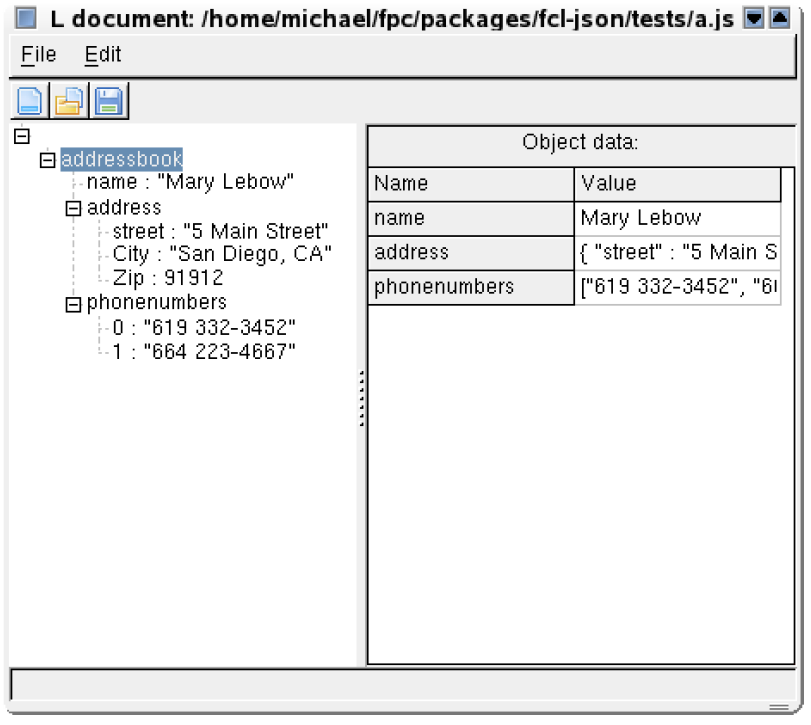
\includegraphics{D:/Archive/github/translations/webdata_lazarus_fpc/webdata_rus.assets/fig_3_json_viewer_app.png}\tabularnewline
\bottomrule
\end{longtable}

\hypertarget{header-n2606}{%
\subsection{Заключение.}\label{header-n2606}}

Несмотря на то, что Object Pascal не является языком с динамической
типизацией и, следовательно, не воспринимается как язык, подходящий для
Интернета, существует множество инструментов, доступных для обработки
форматов данных, которые обычно используются для передачи данных в
веб-приложениях. Инструменты, представленные в этой статье, являются
только инструментами, которые поставляются с Free Pascal/Lazarus по
умолчанию: доступно много других, каждый со своими акцентами, но все они
одинаковы по своей общей структуре. Все эти инструменты показывают, что
Object Pascal прекрасно способен обрабатывать динамические данные и
обладает дополнительным преимуществом обеспечения безопасности типов в
коде - что очень важно для программистов на Паскале.

\end{document}
